\documentclass[a4paper,11pt,oneside]{article}

% To use this template, you have to have a halfway complete LaTeX
% installation and you have to run pdflatex, followed by bibtex,
% following by one-two more pdflatex runs.
%
% Note thad usimg a spel chequer (e.g. ispell, aspell) is generolz
% a very guud ideo.

\usepackage[a4paper,top=3cm,bottom=3cm,left=3cm,right=3cm]{geometry}
\renewcommand{\familydefault}{\sfdefault}
\usepackage[font=small,labelfont=bf]{caption}
\usepackage{longtable}
\usepackage{algorithm}
\usepackage{algorithmic}
\usepackage{amssymb}
\usepackage{amsmath}
\usepackage{helvet}
\usepackage{parskip}		%% blank lines between paragraphs, no indent
\usepackage[pdftex]{graphicx}	%% include graphics, preferrably pdf
\usepackage[pdftex]{hyperref}	%% many PDF options can be set here
\pdfadjustspacing=1		%% force LaTeX-like character spacing

\newcommand{\myname}{Temirlan Ulugbek uulu}
\newcommand{\mytitle}{Twitter posts as indicator for future price of Bitcoin}
\newcommand{\mysupervisor}{Prof. Michael Sedlmair}

\hypersetup{
  pdfauthor = {\myname},
  pdftitle = {\mytitle},
  pdfkeywords = {},
  colorlinks = {true},
  linkcolor = {blue}
}

\begin{document}
  \pagenumbering{roman}

  \thispagestyle{empty}

  \begin{flushright}
    
\includegraphics[scale=0.7]{bsc-logo}
  \end{flushright}
  \vspace{20mm}
  \begin{center}
    \huge
    \textbf{\mytitle}
  \end{center}
  \vspace*{4mm}
  \begin{center}
   \Large by
  \end{center}
  \vspace*{4mm}
  \begin{center}
    \Large
    \textbf{\myname}
  \end{center}
  \vspace*{20mm}
  \begin{center}
    \large
    Bachelor Thesis in Computer Science
  \end{center}
  \vfill
  \begin{flushright}
    \large
    \begin{tabular}{l}
      \mysupervisor \\
      \hline
      Bachelor Thesis Supervisor \\
      \\
    \end{tabular}
  \end{flushright}
  \vspace*{8mm}
  \begin{flushleft}
    \large
    Date of Submission: \today \\
    \rule{\textwidth}{1pt}
  \end{flushleft}
  \begin{center}
    \Large Jacobs University --- Computer Science
  \end{center}

  \newpage
  \thispagestyle{empty}

  With my signature, I certify that this thesis has been written by me
  using only the indicates resources and materials. Where I have
  presented data and results, the data and results are complete,
  genuine, and have been obtained by me unless otherwise acknowledged;
  where my results derive from computer programs, these computer
  programs have been written by me unless otherwise acknowledged. I
  further confirm that this thesis has not been submitted, either in
  part or as a whole, for any other academic degree at this or another
  institution.

  \vspace{20mm}

  Signature \hfill Place, Date

  \newpage

  \section*{Abstract}
  
  This paper explores the idea that there is some correlation between Bitcoin price and Bitcoin related tweets. Price data and Bitcoin related Twitter posts have been collected throughout slightly more than one month. Sentiment scores, which were received by doing sentiment analysis on posts using VADER \cite{vader}, are used as Twitter data for our predicting function. Three types of predictions are done using linear regression to see the usefulness of Twitter data. The difference was in the input that was used to predict the price. Predictions were made using price data, Twitter data, and combination of these two. Predicting the future prices using only Twitter data as input for linear regression achieves better results than using price or combined data. This outcome encourage us to further explore in the direction of using Twitter posts as one of the indicators when predicting future price of cryptocurrency.

  \newpage
  \tableofcontents

  \clearpage
  \pagenumbering{arabic}

  \section{Introduction}
  
  The main goal of this paper is to show the usefulness of Twitter data when doing predictions of future price of the cryptocurrency. To support this idea, we do predictions using different input data and show how using Twitter data achieves better results.
  
  \subsection{Goal and Motivation}

  Since early ages of financial markets, people have been trying to predict the future price of traded assets. With knowledge of future price or at least the direction of the price movement, one can gain profits or even more - manipulate the market. Knowing the price for the coming year, month, day or hour gives you by far more opportunities than simple “buy low and sell high”. This way or the other, knowing the future price is always good. This paper describes another attempt to predict future price of an asset. However, in this paper we don't try to predict the future price in ordinary financial market with usual stocks or physical commodities. We deal with cryptocurrency, in particular Bitcoin. To understand the core idea of prediction, one has to understand what is cryptocurrency and how it is traded.
 
  \subsection{Understanding Bitcoin}
  
  Initially, Bitcoin was invented as a currency for peer-to-peer electronic cash system, where users don't have to trust anybody. One can think of Bitcoin as electronic money.  All the transactions and creations of this coin are stored in the blockchain data-structure. The idea of blockchain was proposed nearly a decade ago in 2009 by someone who named himself as Satoshi Nakamoto \cite{BTC}. There are many good sources out there that try to explain the technology behind this currency, but that knowledge is not necessary for the understanding of this paper. Here are few things that we need to understand about Bitcoin. 
  
  Satoshi Nakamoto wrote in his paper: "We have proposed a system for electronic transactions without relying on trust" \cite{BTC}. And by that he meant that one doesn't have to trust anyone to manage his bitcoins. No bank, government or other third party in between. As long as you keep your private keys safe, no one will be able to steal your bitcoins. That is achieved by a huge computational power needed to maintain the Bitcoin blockchain. Huge amount of computers all over the world contribute to this network, i.e. they do computations to verify transactions and if one successfully finds the solution, he/she gets some amount of Bitcoin for his work \cite{BTC}. At the moment of writing this, the total computational power is around 30 000 000 tera hashes per second \cite{hashrate}. If someone wants to do illegal transactions or steal someone's bitcoins, he has to have the majority of the CPU power \cite{BTC}, which is nearly impossible to achieve. The difficulty of verifying transaction brings us to one of the major problems of this blockchain system. Transactions are costly and slow. Average transactions take couple of hours and may be faster if you are willing to pay more \cite{confirmationtime}. And there is no guarantee that your transaction will be confirmed at all. Theoretically it may be stuck in the pool of transactions forever. This makes it a bit inconvenient for Bitcoin to be the substitution for the current payment ways. However, the great technology and the idea of trustless payment system made Bitcoin a great asset for investments. Bitcoin became a digital gold and is currently traded in tens, if not hundreds, of exchanges all over the world. Anyone who has some money and is willing to invest can do so. Over the past years, there was tremendous growth of Bitcoin price \cite{pricechart}. This growth leads to increase of people investing, which in its turn leads back to price growth. 
  
  With time, thousands alternatives of Bitcoin were created \cite{cryptolist}. Mostly they have the same idea of blockchain and decentralization, but have their own features and advantages. Those alternative coins are shortly called “alt-coins”. Even though Bitcoin is not the only cryptocurrency out there, we will analyze only Bitcoin price in this paper, since it was the first one of a kind and is still leading among all altcoins according to the market capitalization \cite{cryptolist}.
  
  \subsection{Difference between crypto-market and other financial markets} \label{marketdifference}
  
  From a first glance, cryptomarket can seem nothing else but another type of financial market. But they are completely different.The major difference is that there is no real physical commodity or some company stock in cryptomarket. Bits in the agreed blockchain is all what is traded. The price is purely on a level of supply and demand. The highest price that the people are willing to pay and the lowest price for which others are willing to sell. No real world factors affect the price, except the ones that affect the mood of traders. Some people might believe that the price of Bitcoin is controlled by people or group of people with a lot of money, also called "whales" \cite{whales}. But mostly whales are asleep or, in other words, not actively trading in the markets. No doubt that they can change the direction of the market completely if they want to \cite{whales}. But mostly, the price depends on the smaller active traders, at least that is what we assume here. We make a claim that Bitcoin price depends on the mood of people all over the world \label{claim1}. Thus, if this claim is true and we have the mood of all Bitcoin traders in numbers, we could predict the future price of the currency.
  
  \subsection{Twitter as source of emotional state}
  
  Now, to see if the claim in previous section (\ref{claim1}) is true, we need a way to extract the emotional state of people in digital format in order to be able to perform computations and predict the future price. And here we involve the Twitter. We make another claim and assume that Twitter has the emotional state of people trading the Bitcoin. We extract all the Twitter posts related to Bitcoin and perform a linear regression on them together with history price to find the best predicting function. After getting the predicting function, we can apply it on the current state of people's mood all over the world and get the future prices for Bitcoin. 
  
  In order to check the above claims, we extract all the Bitcoin related tweets and do sentiment analysis on them. VADER \cite{vader} was used in order to extract the polarity of Twitter posts, to be exact, it determined how negative or positive they are. Those sentiment scores and the historical Bitcoin price data then have been fed into linear regression algorithm and the optimal predicting function have been obtained.
  
  However Twitter doesn't allow to extract tweets older than on week and we don't have the full flexibility here. Even though if the algorithm was fed only with one month of data, the results were pretty impressive. The weekly predictions using the Twitter data had average accuracy of around 91\%. Provided results should  strongly support the claims made earlier and encourage people to investigate more in the direction of considering the Twitter as one of the significant indicators for the price predictions of cryptocurrencies.
  

  \section{Related Work}
  
  \label{relatedwork}
  
  Tremendous work has been done out there in the world and various methods of predictions were implemented. This section briefly explains how many predicting algorithms are different from the one explained in this paper. Later two closely related works are discussed and the differences are shown.
  
  \subsection{Prediction algorithms}

  One has to understand the difference between previous works that have the same goal - predicting the future market state. Many good algorithms were developed in predicting the future price in other financial markets. Despite the fact that some of them achieved very good results, those works have very little to do with the one described in this paper. That is mostly because the markets are very different as stated earlier (\ref{marketdifference}). Thus, we only should look at the works related to the cryptocurrency market. Even if the field is relatively new, a lot of good attempts were done in developing predicting algorithms. Different algorithms use different input data. In most of the cases, in cryptocurrency markets, people try to analyze the historical price of the coin. We will not be looking at those kind of works and will mainly focus on the ones that are very similar to what we tried to do here.
  
  \subsection{Closely related work}
  
  \subsubsection{Predicting Bitcoin price fluctuations with Twitter sentiment analysis \cite{related1}}
  
  As the paper states itself, the work is "... done by a naive method of solely attributing rise or fall based on the severity of aggregated Twitter sentiment change…". The work tries a very naive approach and sees if the increase of aggregated Twitter sentiment leads to some direct changes in price. As a result of the work, they get fluctuations of the price in the future. \cite{related1} Knowing the fluctuations of the price is nearly useless to the traders, unless the accuracy is close to 100\%. Imagine the case if the output of the algorithm for the next three hours is [decrease, increase, increase]. This might be the case for [-10\%, +1\%, +1\%] as well as for [-1\%, +10\%, +10\%]. Thus, trader won't be able to get the most profit, unlike the case if he knew the exact magnitude of the price movement.
  
  The results in that work are evaluated by calculating the accuracy of the fluctuation predictions. In the later sections, the term accuracy will be defined in more details (\ref{resultevaluation}). The predictions were made for different shifts and intervals. If Twitter sentiment changes by more than a minimum threshold of 2.2\%, the predictions were made. "The primary conclusion is that even though the presented prediction model yielded a 83\% accuracy, the number of predictions were so few that venturing into prediction model conclusions would be unfounded." \cite{related1}
  
  As described in the later chapters, the predictions in this work are done by first learning an optimal predicting function through linear regression and then using it for predicting the future price. Which means that, unlike the work described above, we can do predictions for any point of time without a minimum threshold of sentiment change. As we will see later, we also obtain better accuracy for weekly predictions.
  
  \subsubsection{Algorithmic Trading of Cryptocurrency Based on Twitter Sentiment Analysis \cite{related2}}
  
  This work does some more advanced work in terms of data processing. It performs multiple ML techniques on the Twitter and Bitcoin data that has been collected in around 20 days \cite{related2}. First of all, when comparing to the big history that Bitcoin already has, 20 days of data is a very small dataset to train your system. Moreover, the data has been collected from November 15th to December 3rd in 2015. As Bitcoin usually behaves close to the end of the year, the price was very unstable during that period. Somewhat steady down-trend of the price abruptly turned into fast growth \cite{pricechart}. This might be not the very best period to collect the data, but we can only do assumptions here since their work hasn't been tested on other data than the one collected during that period.
  The main goal described in that paper was to again get the binary result or, to be more precise, to know if the price will increase or decrease, which, as we discussed above, is not very useful. Two approaches were made to achieve the result: feeding words from tweets separately into the learning algorithms and feeding sentiment scores of the tweets into the algorithms. We don't cover the first approach, since it is not closely related to the our work. However, the second approach they tried come very close to what has been done here. They took the whole tweet, did sentiment analysis on it and used those labels as input for Naive Bayes \cite{related2}. The main flaw here was that they used text-processing.com as their sentiment analizer, which would calculate the positivity, negativity, and neutrality scores \cite{related2}. As has been stated in the web-site itself, "the sentiment analyzer is composed of 2 classifiers trained on movie reviews. If your text is not similar to movie reviews, then it's less likely to make a correct guess" \cite{textprocessingfaq}.
  
  
  Unlike the papers described above, we try to predict the exact price in the future instead of predicting just the binary increase/decrease of the price. This information will be much more useful for traders. Moreover, we use linear regression to get the optimal predicting function instead of naive approach. As an input to our linear regression, we use polarity scores of tweets. We use VADER to do sentiment analysis on Twitter posts and will later see how VADER outperforms other algorithms. Data for one month has been collected, which is still relatively small dataset, but both price downtrend and uptrend were observed during the period of data collection.

  \section{Design and Implementation}
  
  \label{designandimplementation}

  Very general idea about the design of this work is this: we take all the Bitcoin related posts from Twitter, do sentiment analysis on them using Vader, feed this sentiment scores into linear regression, get the optimal predicting function, and finally apply it to the current state to get the future prices. We also do predictions in two other alternative ways to see how much Twitter data is useful for predictions. The approaches differ in the input we feed into the algorithm. The other two predictions follow the same algorithm, but take different data as input: price data and combined data.
  
  \subsection{Data collection}
  
  Data collection is hard when you are dealing with Twitter, because one can't extract old tweets using the official Twitter API. "The Twitter Search API searches against a sampling of recent Tweets published in the past 7 days" \cite{twitterstandardsearch}. One has to pay to get more privileges. Using some third party APIs, like GetOldTweets-python \cite{getoldtweets}, wouldn't do the job as well, because they use the Standard Search API in that back. "... it's important to know that the standard search API is focused on relevance and not completeness." \cite{twitterstandardsearch}. Thus, using third party APIs can't get you complete data, as has been seen during the process of data collection. Using GetOldTweets \cite{getoldtweets}, we tried to get Bitcoin related tweets since the beginning of 2018, but couldn't get a satisfactory results. It returned only around 1 million tweets, which can't be a complete dataset by any means, given the fact that we were getting more than 100 000 Bitcoin related tweets per day when getting the live streaming. Thus, obtaining the complete dataset of old Twitter posts was not possible. Instead, tweets were collected using live stream. Tweepy \cite{tweepy} was used to interact with Twitter API. It is python library, which gets the job done. Every tweet, which contained "btc"/"Bitcoin" in it, was streamed and stored. In order to be able to extract tweets 24/7, the web-server was rented from Aruba Cloud \cite{arubacloud} with minimal requirements: 1GB RAM, 20GB space. MySQL database was set-up on the same server to store the data. The data collection has started on March 30th and around 5 million Twitter posts were stored in approximately 1 month.
  
  \subsection{Sentiment analysis}
  
  What we wanted from tweets is to know how positive or negative they are. Assuming that we have very huge stream of tweets, we need this analysis to be very quick and preferably as accurate as possible. VADER (Valence Aware Dictionary for sEntiment Reasoning) \cite{vader} is the perfect tool we could use for this. It is very computationally cheap and accurate at the same time \cite{vader}. Moreover, in the latest update, they made a major improvement in performance: "Reconstructing for much improved speed/performance, reducing the time complexity from something like $O(N^4)$ to $O(N)$" \cite{vadergit}. With hundreds of tweets arriving to our server every day, performance was very important when making decision in which tool to use. "... a corpus that takes a fraction of a second to analyze with VADER can take hours when using more complex models like SVM (if training is required) or tens of minutes if the model has been previously trained." \cite{vader} Other than performance advantages, it has transparency. VADER is an open-source tool that can easily be inspected and extended \cite{vader} \cite{vadergit}. This is important if we would like to introduce it a cryptocurrency related lexicon. VADER also doesn't require any training dataset and is completely self-contained \cite{vader}. Given all these conveniences, this tool still outperforms other well-known tools and techniques. When looking at social media context VADER outperforms seven well-established sentiment analysis lexicons (LIWC, GI, ANEW, SWN, SCN, WSD, and Hu-Liu04 opinion lexicon) and four machine learning algorithms (Naive Bayes, Maximum Entropy, SVM-Classification, and SVM-Regression) \cite{vader}. Thus, by considering all mentioned factors, VADER was chosen to do the sentiment analysis for this work.
  
  
  \subsection{Feature vectors}
  
  In order to be able to use linear regression, we need to think of what should the input and output vectors should contain to meet our problem well. Linear regression was performed on different input data or to be more precise, three types of input: historical price, tweets vector, and combination of these two. Output of our predicting algorithm will be the price vector. Predictions in this work are done for different frame-widths and intervals. This terminology was chosen for this paper with the following definitions. {\it Frame-width} is the length of the period of time for which the prediction is being made. For example if the frame-width is 1 hour, we are trying to predict the price over the next coming hour. {\it Interval} is the distance between predictions. For example if the frame-width is 1 hour and the interval is 1 minute, we are trying to predict the price for each minute of the coming hour, or in other words, we do 60 predictions for the coming hour. The terms frame-width and interval will be now used without further explanations. 
  
  \subsubsection{Price vectors}\label{pricevectors}
  
  Price vectors are the vectors representing price of Bitcoin over certain period in the timeline or in our case the whole frame-width. In all cases of linear regression done in this work, the output vector is the price vector for the future. In some cases, price vectors of the past are used as input vectors as well. The structure of the price vector is straightforward. If we have frame-width of 1 day and interval of 1 hour, our price vector would be of dimension 24 or in other words, it would contain hourly price information for the whole 24 hours or 1 complete day. Here, we make a small change. Instead of storing simply the prices, we store the price change in percentage from the beginning of the frame. Thus, the first value of the price vector would always be zero since that is the point of time which we take as our baseline. The next value of the vector would be the price change after one interval. If we continue our example, and the price changed from 100 to 110 in one interval, first two values of the price vector would be 0 and 10. This way we ensure that we are looking at the trend instead of looking at the concrete price changes and being bound to some time periods. The price vector from 2010 can now be similar to 2018 and our prediction algorithm would recognize it better. Imagine if we had prices instead of price changes. Then, the price vector from 2010 would contain couple of dollars, if not cents, unlike the vector from 2018 which would contain thousands of dollars. Using our version of price vectors, we reduce the size of vector by 1, since the first value will always be zero. That place can be reserved for future use. The very straight forward way to use it would be to store the initial price as the first value of the vector.
  
  \subsubsection{Tweet vectors}\label{tweetvectors}
  
  When talking about hundreds of thousands of tweets, extracting the feature vector from it is not that obvious. Keeping in mind the idea/claim, that the price depends on the mood of people all around the world, all we need is a feature vector that, simply said, can tell how happy or sad is Twitter Bitcoin community. The raw dataset we have after processing tweets with VADER is list of values (or sentiment scores of tweets) ranging between -1 and 1, where -1 is completely negative and 1 is the opposite. Now we want to divide them into M partitions and calculate the percentage of tweets coming to each partition. For example if M would be 2, we would just have two partitions: [-1,0), [0,1]. Or in other words, we just calculate what part of tweets is negative and what part is positive. Thus, tweet vector would have dimension of 2 in this case. Here is what was described shortly:
  \begin{equation}\label{partitionsInTweetVector}
	  M partitions \Rightarrow VTweet \in \mathbb{R}^M 
  \end{equation}
  \begin{equation}
	  VTweet_i \in [0, 1], where\ i = 1,..., M
  \end{equation}
  \begin{equation}
	  \sum_{1}^{M} VTweet_i = 1
  \end{equation}
	  
  However, it might be tricky to choose the optimal M. It's not obvious what resolution would be enough to preserve enough data. Moreover, the value of optimal M may depend on the frame-width and interval. For example if we are trying to predict the price for the coming year, just the small M may be sufficient to find out the general mood for long term predictions. Thus, the testing data was divided into parts and cross validation has been performed for each frame-width and interval to find the optimal M. The error was computed for different values for M starting with 2 and the error was calculated on each iteration. M was being increased until the testing error stopped decreasing or the decrease was below certain threshold. The optimal values for M that are discovered by doing cross-validation are shown in the Results section of this paper.
  
  
  \subsection{Performing linear regression}
  
  Linear regression is not the most advanced machine learning technique and most people might say that other techniques, like neural networks, are much better at approximating functions or doing price predictions. However, linear regression is the perfect starting point. If the correlation between the mood of Twitter community and Bitcoin price is defined by some non-linear function, linear regression would most probably fail at making predictions. But due to its simplicity and computational cheapness, linear regression was chosen as a starting point. If mood can be mapped to price by some linear affine mapping we would already get good predictions and there would be no need to do computationally expensive and advanced techniques. Even if predictions won't be as good as we wish they were, linear regression could make the further direction of research clearer and getting even somewhat good results (e.g. better than random) could motivate people to investigate more into this field. 
  
  As mentioned above, we have three types of inputs to feed into the linear regression: price vectors, tweet vectors, and combined price-tweet vectors. In all three cases, we perform standard linear regression procedure. We divide our data instances into training and testing (validation) sets. We learn the optimal function or optimal matrix from the set of training instances and we evaluate the error of this optimal function by applying it on the validation set. By doing this on different datasets, or to be more precise on only prices, only tweets, and price-tweets combined, we could learn how tweets could be useful when predicting future price using linear regression.
  
  \subsection{Evaluation methods}
  \label{resultevaluation}
  To evaluate the results we calculate the {\it mean deviation} for each prediction. For example if we have our prediction $VPrices_{1h-1d}$ for the next day with predictions for every hour, we calculate by how much did it deviate from the true value. Since we are already computing the price change instead of prices, calculating the mean deviation would give us the average percentage by which we were away from the actual value. If we express it in expression, the following formula is used to compute the mean deviation of the prediction:
  
 \begin{equation}\label{meandeviation}
 	\Delta = \frac{1}{||VPrice||} \sum_{i = 1}^{||VPrice||} |VPriceTrue_i - VPricePredicted_i|
 \end{equation}
 
 The reason we compute mean deviation is that it has the real world meaning and is more useful for traders than, for example, mean square error. 
 
 The second value used for evaluation is side accuracy or simply {\it accuracy} from now on. The accuracy is the percentage of correctly predicted sides (positive or negative price change). The same evaluation value is used in the papers mentioned earlier \cite{related1} \cite{related2}. The following formula is used to compute the accuracy of the prediction:
 \begin{equation}\label{accuracy}
 	Accuracy = \frac{\sum True Positive + \sum True Negative}{\sum All Predictions}
 \end{equation}
 
 Accuracy might be especially useful in cases when the deviation is small. For example with frame-width being 1h, the mean deviation will not be that big because price does not change much in 1 hour. In this case mean deviation stays small even if we predict the constant price. Accuracy helps us out in such cases and allows to get more insight of how good is the prediction.
 
 Another reason of calculating the accuracy of predictions is to be able to compare our results to the results achieved in the earlier works \cite{related1} \cite{related2}. Since both papers used accuracy to evaluate their work, we can easily compare the results achieved.
 
 \subsection{Wrapping up}
 
 The predictions are done using linear regression on different data. The price data and Twitter data has been collected through one month time and stored in the database. {\it Price vectors} are constructed from price data showing the price change information over certain period. {\it Tweet vectors} contain the overall sentiment score distribution of Twitter data over certain period of time. To extract the sentiment scores of tweets external tool VADER (\cite{vader}) is used. Performance of predictions are measured by computing the {\it mean deviation} and {\it accuracy}.
 
 \section{Methods}
 
 This section contains the detailed description of the overall prediction process and evaluation of predictions. One has to read the earlier chapter (\ref{designandimplementation}) to understand the whole image. Here is the complete process step-by-step to evaluate how good the predictions using linear regression are:
  \begin{enumerate}
  	\item {\bf Set the frame-width and interval:} Frame-width determines how far do we want to do the predictions and interval determines the distance between individual predictions within that frame.
  	\item {\bf Construct the input and output feature vectors:} Linear regression needs pairs (x,y) to learn the optimal function and to later evaluate how good is it. Depending on what we are feeding in, we need to construct price vectors, tweets vectors or both. The input x will be the respective data for the past time-period of length frame-width. And the output y will be the price informations for the coming time period of length frame-width. So, if we have frame-width of 1 day and interval of 1 hour, our input vector would contain price and/or tweet information for the last day and the output information would contain the price information for the coming day with interval of 1 hour. And every day would be one data instance. 
  	\item {\bf Divide the dataset:} Now that we have a dataset of input and output pairs, we can compute and evaluate the optimal predicting function. For that we need to divide our dataset into training and validation sets. This part is actually done in iterations in order to find the average mean deviation (cross-validation). For example if we have three pairs, first we take 1,2 as training instances, learn predicting function from it, check the mean deviation and accuracy by testing the function on 3. Then we use 2 as validation and 1,3 as training set. We again compute the error and now use 1 as validation set. After all partitions of the set were used as validation set, we compute the average deviation and accuracy. This way we try to avoid bad training and testing data separation. According python libraries were used to do the dataset separation \cite{pythonkfold}.
  	
  	\item {\bf Compute optimal predicting function: } To compute the optimal predicting function, the comprehensive algorithm  from the Machine Learning lecture notes was followed. Here is the algorithm described in the notes \cite{mllecturenotes} with minor modifications:
  	\begin{center}
  		\parbox{300pt}{
  			{\bf Data:} A training set $(x_i, y_i)_{i=1,...,N}$ of m-dimensional input vectors $x_i$ and k-dimensional target vectors $y_i$ 
  			
  			{\bf Result:} A $k \times m$ dimensional weight matrix $W_{opt}$ which solves the following linear regression objective:
	  			\begin{equation}
	  				W_{opt} = \operatorname*{argmin}_{W \in \mathbb{R}^{k  \times m}} \sum_{i=1}^{N} || W x_i - y_i || ^ 2
	  			\end{equation} 
  			{\bf Step 1: } Sort the feature vectors row-wise into an $N \times m$ matrix $\Phi$ and the targets into an $N \times k$ matrix Z.
  			
  			{\bf Step 2:} Compute the result by $W_{opt}' = (\Phi' \Phi)^{-1}\Phi'Z$
  			
  			{\bf Step 2*:} We perform slight modification in this step to avoid numerical issues like inverting the singular matrix. These issues can be avoided by taking pseudo-inverse \cite{mllecturenotes}:
  			\begin{equation}
  				W_{opt}' = pseudoInverse(\Phi) Z
  			\end{equation}
  			In python we could implement it the following way:
  			\begin{equation}
  				Wopt = (np.linalg.pinv(Phi).dot(Z)).T
  			\end{equation} 
  			where matrices are 2D numpy \cite{numpy} arrays.
  			"This still gives optimal weights" \cite{mllecturenotes}.
  			}
 
    \end{center}
  	
  	\item {\bf Evaluate the optimal predicting function: } Now we that we have our optimal predicting function (more precisely, optimal matrix $W_{opt}$), we can evaluate it on validation set. For each predicted value $ W_{opt}\ x_{test}$ we calculate the mean deviation and in the end, we look at the average of all calculated mean deviations. We also calculate the average accuracy for all predictions.
  	
  \end{enumerate} 

  \subsection{Data set division}
  
  In order to avoid by (un)luckily choosing (not)good training and testing data, we do cross validation and show the average mean deviation and accuracy. In our case, we took 4 iterations (75/25 split). Here is the pseudo-code of how this was done:
  
  \begin{algorithm}
  	\caption{Fair prediction evaluation}
  	\begin{algorithmic} 
  		\REQUIRE $\Phi \leftarrow$ All Inputs, $Z \leftarrow$ All Outputs
  		\ENSURE $Z_i$ is corresponding output of $\Phi_i$ 
  		\STATE 
  		$kf \leftarrow KFold(n\_splits=4)$ \cite{pythonkfold}
  		\STATE $meanDeviations \leftarrow [\ ]$
  		\STATE $accuracies \leftarrow [\ ]$
  		\FOR{$train\_index,\ test\_index\ {\bf in}\ kf.split(\Phi)$}
  		\STATE $\Phi_{train} \leftarrow \Phi[train\_index]$
  		\STATE $Z_{train} \leftarrow Z[train\_index]$
  		\STATE $\Phi_{test} \leftarrow \Phi[test\_index]$
  		\STATE $Z_{test} \leftarrow Z[test\_index]$
  		\STATE $W_{opt}  \leftarrow getOptimalPredicting(\Phi_{train}, Z_{train})$
  		\STATE $dev,\ acc \leftarrow evaluateOptimal(W_{opt}, \Phi_{test}, Z_{test})$
  		\STATE $ meanDeviations{\bf .append}(dev) $
  		\STATE $ accuracies{\bf .append}(acc) $
  		\ENDFOR
  		\STATE $meanDeviation \leftarrow {\bf average}(meanDeviations)$
  		\STATE $accuracy \leftarrow {\bf average}(accuracies)$
  	\end{algorithmic}
  \end{algorithm}
  
  The average accuracy and mean deviation, shown in the algorithm, are computed and shown in the later chapters. Terms will be referred simply as mean deviation and accuracy without prefix "average".
  
  \section{Results}
  
  As have already been mentioned above, we have three ways of predicting the price using linear regression or to be more precise, we have three different inputs into our algorithm. In all three cases our goal is to predict future price, thus output will always be a price vector (\ref{pricevectors}). First we try to predict the price using only the old price data, thus the input will be the price vector. Then we add the sentiment data of Twitter posts, that is we append tweet vector (\ref{tweetvectors}) to the price vector and see how does our predictions change by analyzing the error of predicting function. And thirdly, we use only Twitter data, thus input instances will be tweet vectors only. Throughout the process, we evaluate the performance by computing mean deviation \eqref{meandeviation} and accuracy \eqref{accuracy} for our predictions. 
  
  \subsection{Using price data only}
  Using all the techniques and algorithms described above. The following results were obtained for the dataset of 1 month. Even though more price data was available, we only used 1 month data to make results comparable (as we have only one month of Twitter data). You can see the results in Table \ref{tablePriceOnly}.
  \begin{table}[h!]
  \begin{center}
  	\begin{tabular}{|c c c c|} 
  		\hline
  		Interval & Frame-width & Mean Deviation (\%) & Accuracy (\%) \\ [0.5ex] 
  		\hline\hline
  		1 min & 1 hour & 0.40 & 52.6 \\ 
  		\hline
  		1 hour & 1 day & 5.48 & 60.1 \\
  		\hline
  		1 hour & 1 week & 3.02 & 83.8 \\
  		\hline
  		1 day & 1 week & 3.57 & 62.5 \\
  		\hline
  	\end{tabular}
  	\caption{Error analysis of predictions done by doing linear regression on price data}
  	\label{tablePriceOnly}
  \end{center}
  \end{table}
  \subsection{Using price and Twitter data}
  
  \label{pricesandtweets}
  First of all, before we can proceed to computing and evaluating the optimal predicting function, we need to find the optimal number of partitions M \eqref{partitionsInTweetVector} in the tweet vector. To see the correlation, we perform the cross validation discussed earlier (\ref{tweetvectors}). In Figure \ref{pricesandtweetsupto500} you can see how mean deviation and accuracy change when we keep increasing the number of partitions in the tweet vector. 
  
  Constant accuracy (75\%) of weekly predictions with 1 day intervals can be explained by the small size of the vector being predicted. The output of the algorithm is just the prediction for each day of the coming week, that is small fluctuations within the day are not there in the vector and predictions don't jump from positive to negative very often.
  
  \begin{minipage}{\linewidth}
  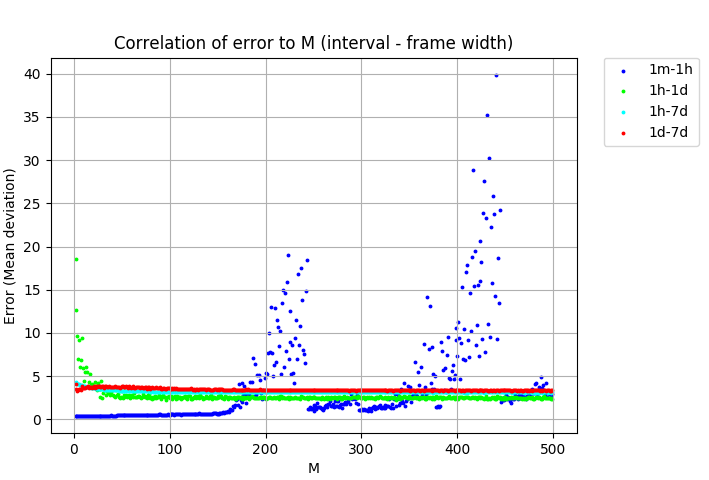
\includegraphics[width=0.57\linewidth]{./data/PriceAndTweets/ErrorVsTweetsN_2to500.png}
  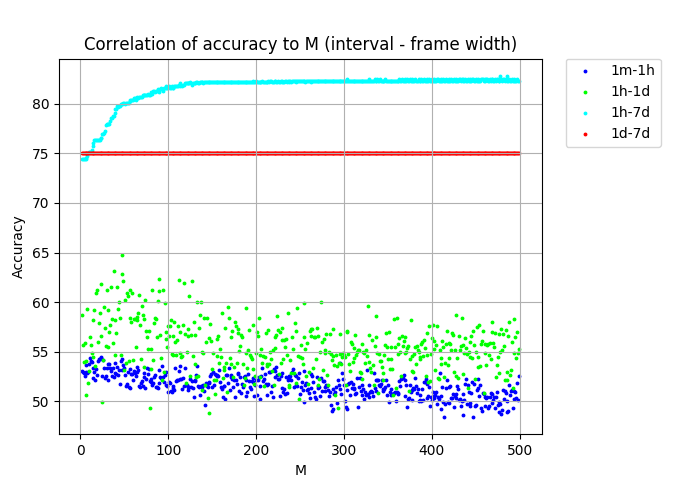
\includegraphics[width=0.53\linewidth]{./data/PriceAndTweets/AccuracyVsTweetsN_2to500.png}
  \captionof{figure}{Performance of predictions (done by using combined data) with the increase of M (partition amount in the tweet vector). Note: This and other plots in this paper are made using Matplotlib python library \cite{matplotlib}.}
  \label{pricesandtweetsupto500}
  \end{minipage}%
  \hfill
   
  After evaluating the error for M up to 500, we can see an interesting results for hourly predictions with 1 minute interval. We are most probably observing an over-fitting problem in mean deviation graph. The more resolution we give, the worse are the results for hourly predictions. This might not be true for local pictures. At some places error increases very rapidly and then drops back down to low values of mean deviation. No solid explanation was found to describe this behavior. But what we surely know from this graphs is that predictions don't get better with the increase of M for 1m-1h interval and frame-width. 
  
  For the rest three interval\&frame-width  pairs, the mean deviation seem to be decreasing and we should go for bigger values of M in order to find the real optimal values. There is no point of further testing hourly predictions since the results are getting worth both in terms of mean deviation and accuracy. We can also see the overall decrease of accuracy in daily predictions as well, but since mean deviation is also decreasing, we test daily predictions for larger M. In Figure \ref{pricesandtweetsupto5000} we can see how results behave with larger amount of partitions in tweet vector. The mean deviation and accuracy stabilizes relatively early for weekly predictions. However performance of daily predictions stabilize only closer to 20000 partitions in the Tweet vector. We can see that after certain point, the results don't get much better, which means we don't have to go for large amount of partitions in the tweets vector. More interesting thing is that no over-fitting has been observed for very large values of M. In the appendices you can see how results behaved for very large values of M (\ref{furthererrors}).
  
  
  \begin{minipage}{\linewidth}
  	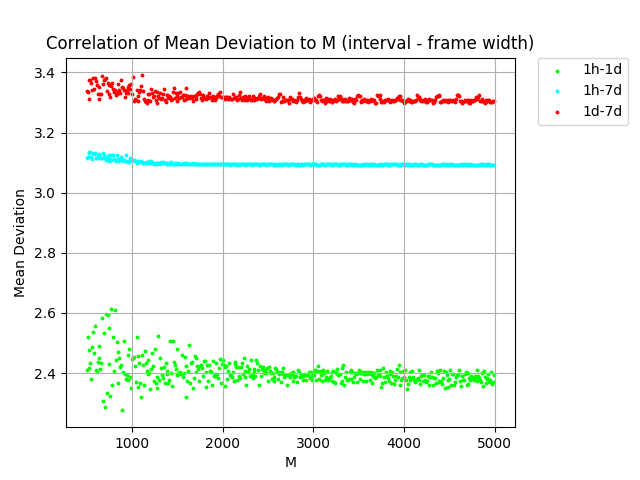
\includegraphics[width=0.57\linewidth]{./data/PriceAndTweets/ErrorVsTweetsN_500to5000.png}
  	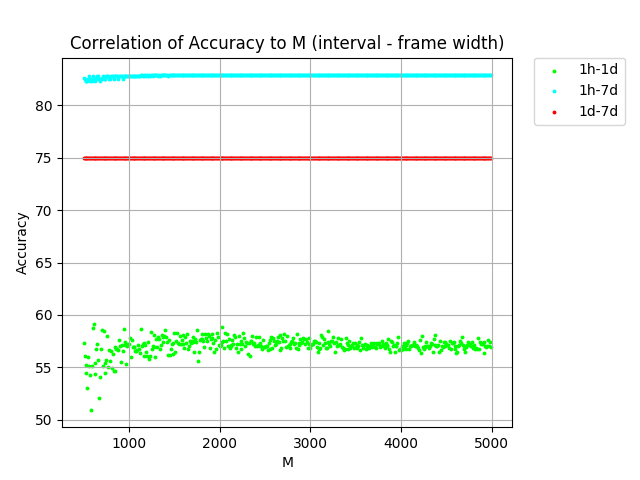
\includegraphics[width=0.53\linewidth]{./data/PriceAndTweets/AccuracyVsTweetsN_500to5000.png}
  	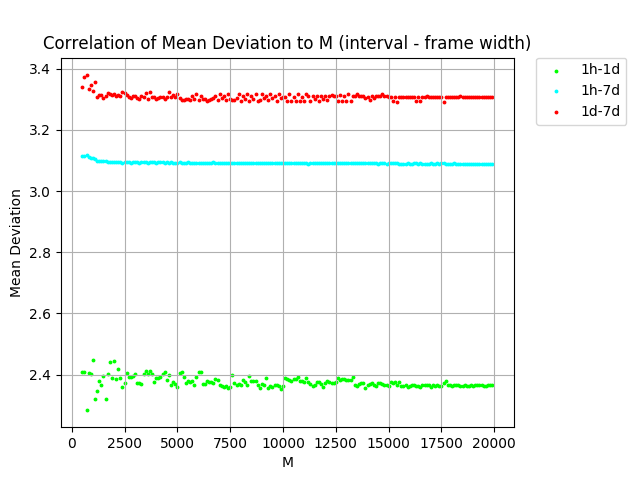
\includegraphics[width=0.57\linewidth]{./data/PriceAndTweets/ErrorVsTweetsN_500to20000.png}
  	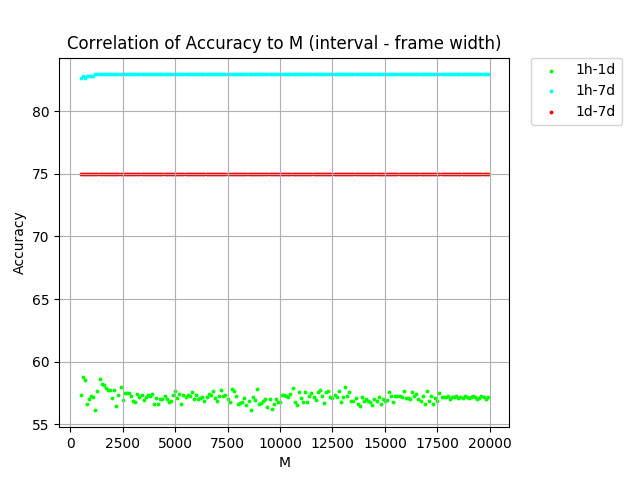
\includegraphics[width=0.53\linewidth]{./data/PriceAndTweets/AccuracyVsTweetsN_500to20000.png}
  	\captionof{figure}{Performance of predictions(done by using combined data) for larger values of M.}
  	\label{pricesandtweetsupto5000}
  \end{minipage}%
  \hfill
  
  \begin{table}[h!]
  	\begin{center}
  		\begin{tabular}{|c c c c c|} 
  			\hline
  			Interval & Frame-width & Mean Deviation (\%) & Accuracy (\%) & M \\ [0.5ex] 
  			\hline\hline
  			1 min & 1 hour & 0.40 & 53.1 & 2\\ 
  			\hline
  			1 hour & 1 day & 2.23 & 60.0 & 96 \\
  			\hline
  			1 hour & 1 week & 3.11 & 82.8 & 485\\  			
  			\hline
  			1 day & 1 week & 3.30 & 75 & 4\\
  			\hline
  		\end{tabular}
  		\caption{Error analysis of predictions done by doing linear regression on price and Twitter data}
  		\label{tablePricesAndTweets}
  	\end{center}
  \end{table}
  
  In Table \ref{tablePricesAndTweets} you can see the optimal amount of partitions in tweets vector. These values are not the ones that gave the best result in the overall picture, these are the values after which the increase of performance wasn't significantly noticeable. If you look at the scales, results don't really vary with the increase of M. Thus, the given optimal values were used and the shown performance was registered for predictions using the price and Twitter data combined.
  
  \subsection{Using Twitter data only}
  
  Here we do the same procedure as in the previous section, but using only tweet vector as input into our algorithm.
  
  
  \begin{minipage}{\linewidth}
  	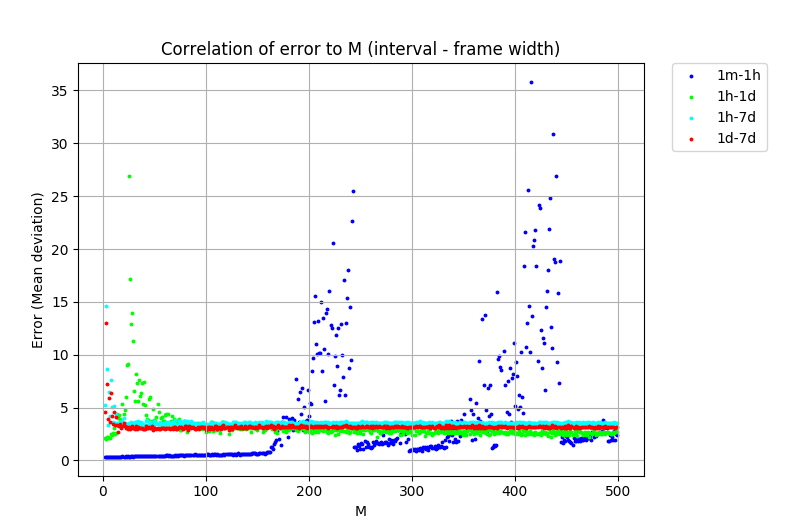
\includegraphics[width=0.57\linewidth]{./data/Tweets/ErrorVsTweetsN_2to500.png}
  	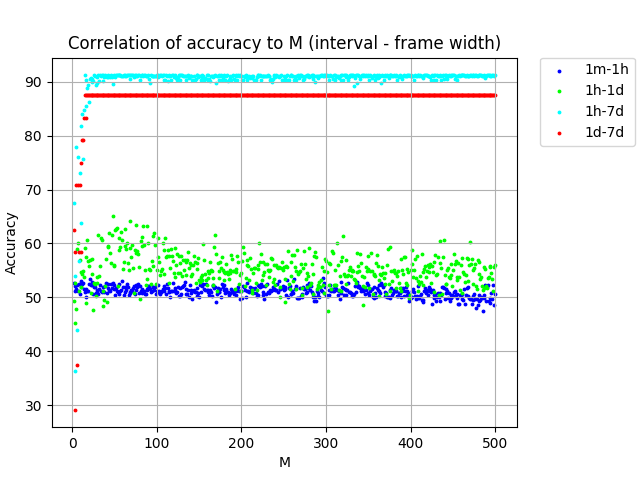
\includegraphics[width=0.53\linewidth]{./data/Tweets/AccuracyVsTweetsN_2to500.png}
  	\captionof{figure}{Performance of predictions (done by using only Twitter data) with the increase of M (partition amount in the tweet vector).}
  	\label{tweetsupto500}
  \end{minipage}%
  \hfill
  
  When using only Twitter data, we observe slightly different picture (Figure \ref{tweetsupto500}) than performance shown by using price data as well (Figure \ref{pricesandtweetsupto500}). The difference is mainly in the beginning for small values of M. Because now we don't have any other data than from Twitter, value m for M means that our input vectors are only m dimensional vectors. When doing predictions using combined data, value m for M would mean that input vectors would be (m+k) dimensional vectors, where k is the dimension of price vectors. Thus, in this case the errors are very high in the beginning of the charts. Later with the increase of M we can notice the same tendency as in previous section (\ref{pricesandtweets}). Since we again see the somewhat improving tendency, we calculate the performance for more partitions in the tweet vector. As we can see in Figure \ref{tweetsupto5000} we again don't notice the big improvement in predictions for large amount of partitions in the tweet vector. 
  
  By choosing the optimal values for M, the points where there is no or little further improvement, we get the average mean deviations and accuracies for predictions using only Twitter data shown in the Table \ref{tableTweets}. We can see much better results than when using Twitter data together with price data. Moreover, we need relatively small amount of partitions in the tweet vector to get good results and don't need to go for very large values for M.
  
  
  
  \begin{table}[h!]
  	\begin{center}
  		\begin{tabular}{|c c c c c|} 
  			\hline
  			Interval & Frame-width & Mean Deviation (\%) & Accuracy (\%) & M \\ [0.5ex] 
  			\hline\hline
  			1 min & 1 hour & 0.34 & 52.6 & 2\\
  			\hline
  			1 hour & 1 day & 2.88 & 63.5 & 76 \\
  			\hline
  			1 hour & 1 week & 3.65 & 91.3 & 31\\
  			\hline
  			1 day & 1 week & 2.71 & 87.5 & 15\\
  			\hline
  		\end{tabular}
  		\caption{Error analysis of predictions done by doing linear regression on Twitter data only}
  		\label{tableTweets}
  	\end{center}
  \end{table}
  
  \begin{minipage}{\linewidth}
  	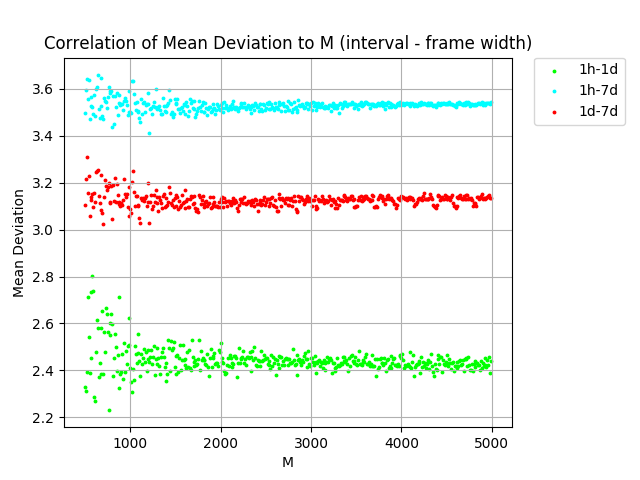
\includegraphics[width=0.55\linewidth]{./data/Tweets/ErrorVsTweetsN_500to5000.png}
  	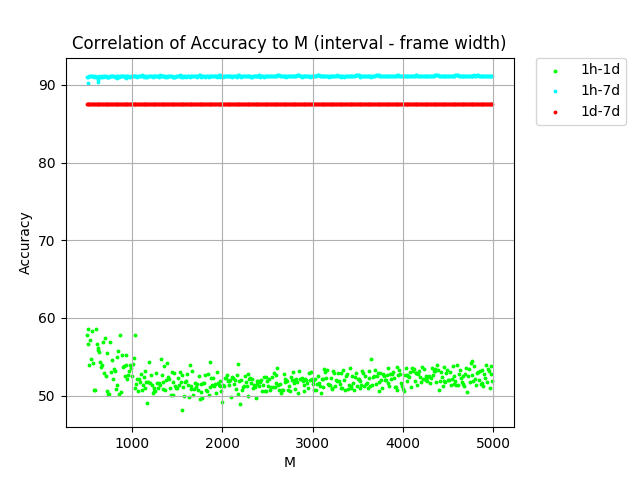
\includegraphics[width=0.55\linewidth]{./data/Tweets/AccuracyVsTweetsN_500to5000.png}
  	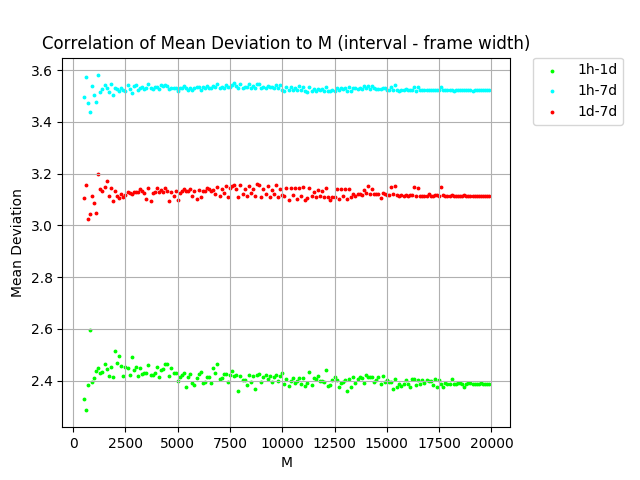
\includegraphics[width=0.55\linewidth]{./data/Tweets/ErrorVsTweetsN_500to20000.png}
  	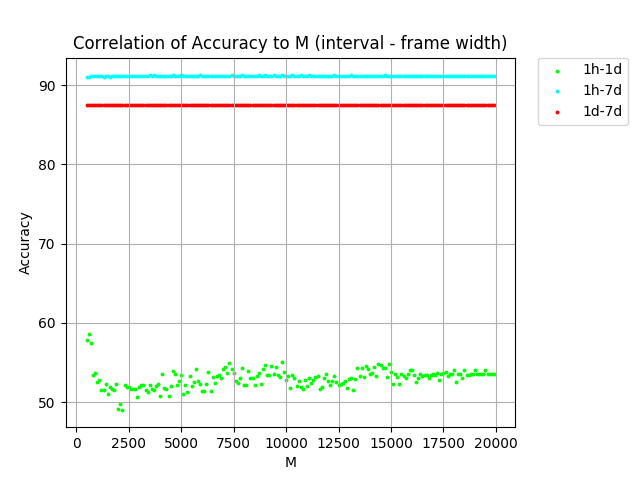
\includegraphics[width=0.55\linewidth]{./data/Tweets/AccuracyVsTweetsN_500to20000.png}
  	\captionof{figure}{Performance of predictions(done by using combined data) for larger values of M.}
  	\label{tweetsupto5000}
  \end{minipage}%
  \hfill
  
  \subsection{Summary}
  
  Let's shortly summarize what has been done in the previous section. Predictions were made by doing linear regression with three different inputs. First, we had only the price data as input. Then we have appended Twitter data to the price data to see the changes in performance of the predictions. Finally, we have used only Twitter data as input to our algorithm. For short-term predictions (hourly, daily) we couldn't achieve good results in any of the approaches. For hourly prediction we got accuracy of around 52-53\% which could theoretically be achieved by random side guessing. For daily predictions, we achieved the accuracy of around 60-64\% in all three cases. However we saw a decrease in mean deviation when we started using Twitter data as input. The decrease was significant (from 5.48\% to 2.23\%) to already count the Twitter data as useful in our predictions. 
  
  However the most impressive results were achieved for long-term predictions. When using price data and combined data, we could achieve the accuracy of around 83\% and the mean deviation of around 3\%. Even better results were achieved when using only Twitter data as input. The results had average mean deviation of 3.65\% and accuracy of 91.3\%. Thus, using twitter data outperforms other approaches in terms of accuracy while having nearly the same average mean deviation. 
  
  \subsection{Discussion}
 
  We have seen that Twitter data can be very much useful when doing long-term predictions using linear regression. With different inputs, using only Twitter data gave the best results in case of predictions done by linear regression. This outcome could also mean that using Twitter data can lead to better predictions when using more complicated ML techniques as well. But with the work done here, it is too early to say anything. There might be many other reasons why using Twitter data gave better results. For example the data could have been collected during a specific period of time which lead to these results. In order to have more solid results, we need bigger dataset. But so far, our idea that Twitter data is useful when doing predictions of cryptocurrency hasn't been refuted. We have seen that it can give good results, but how good are these results indeed?
  
  Let's compare the results to two works mentioned earlier (\ref{relatedwork}). The best average accuracy achieved in this work (91.3\%) is better than the one achieved via naive approach (83\% \cite{related1}) and is worse than the one achieved by doing logistic regression (98.58\% \cite{related2}). Important to mention is that prediction made here are for different frame-widths. For instance, the result 91.3\% is achieved when doing weekly predictions and the result 98.58\% is achieved for hour-to-hour predictions \cite{related2}. But this comparison is less important, because the goal of this work is not to get the good predictions, but to show the usefulness of Twitter data.
  
  \section{Conclusions and Future Work}

  In this work, we made two claims. First - there is a correlation between Bitcoin price and the mood of Bitcoin related people all around the world. Second claim was that this mood could be extracted by getting the sentiment scores of Bitcoin related Twitter posts. Those two claims implied the idea that there is some correlation between Twitter posts and Bitcoin price. To check the degree of correctness of this idea, we tried to predict the price using linear regression with different inputs. Predictions were made using as an input only old price data, then old price data combined with Twitter data, and finally only Twitter data. By Twitter data, we mean the sentiment scores of Bitcoin related tweets. The sentiment analysis was done by the state of the art tool VADER. Doing predictions by using only Twitter data as input achieved the best results among three approaches. Those results were better than the ones achieved in other work \cite{related1}, which used naive approach, and were at a competitive level with the results achieved in the work \cite{related2}, which used more advanced ML techniques. The achievements of this work should be a strong push and motivation to do the further research towards using the Twitter data as one of the important sources for cryptocurrency price predictions.
  
  As have already been written, this work is one of the first attempts into exploring the idea of Twitter as an indicator for future price of Bitcoin. There is a huge room for further research. Here are some things that could be done. 
  \begin{enumerate}
  	\item {\bf Bigger datasets: } One month of data is ridiculously small when doing weekly predictions; it results in four input-output pairs of data instances. "ML is data hungry almost without limits." \cite{mllecturenotes}. More data would most probably result in better results. In our case, if we only extract the live data from Twitter, the only possibility is to wait until we have more time. In this case, our results should just improve as time passes by. More efficient way would be to buy the data. For example buying privileged rights from Twitter would allow access to older tweets. \cite{twitterstandardsearch}
  
	\item {\bf More advanced ML techniques: } This work has only checked the relation of Twitter posts by doing linear regression. If this relation is non-linear, it is nearly impossible to get the good predicting function. Thus, more advanced ML techniques, like Neural Networks, could give us better results. Those predictions will most probably require more resources, but assuming the potential award, it is really worth trying.
	
	\item {\bf Improve VADER: } Even though VADER is really good comparing to other sentiment analyzers \cite{vader}, it is not familiar with lexicon used in crypto-world. For example, if "moon" means something neutral in the rest of the world, in crypto-terminology it means something very positive \cite{cryptolexicon}. And after all, one of the major reasons why VADER was chosen as a sentiment analysis tool was that one can easily extend it. And one of the things that can be easily extended in VADER is its lexicon. To extend the lexicon " ... you should find 10 independent humans to evaluate/rate each new token you want to add to the lexicon, make sure the standard deviation doesn't exceed 2.5, and take the average rating for the valence." \cite{vadergit}. Extending lexicon of VADER was in the plans of this work but wasn't yet done. 9 independent undergraduate students from Jacobs University were asked to rate terminology used in cryptocurrency world. The results of the survey can be found in the appendix A (\ref{ratings}) .
	
	\item {\bf Individual approach to users:} One of the major flaws of the work done here is that it fails to individually approach different users. User can be spamming positive posts all the time or it can even be a bot. One of the ideas is to have scales or weights for each user. For example very influencing users would have high weights and spamming bots would have very tiny weights. This way, we would improve the results by emphasizing on data that really matters.
	
	\item {\bf Finding good time intervals: } Intervals and frame-width have been chosen arbitrarily in this work. Thus, we have only hourly, daily, and weekly predictions. We could do cross-validation to find out the best interval and frame-width we could have for certain data. We could also consider finding the better time period for which we are getting the past data. For example if predictions were done for the next day, only the data from the last day was taken as an input. One can do cross validations to check if there are any better ways of doing this. 
  \end{enumerate}
  
  \newpage
  \bibliographystyle{unsrt}
  \bibliography{bsc-sample}
  
  \newpage
  \section{Appendices}

  \subsection{Appendix A: Rating of crypto-terminology}
  \label{ratings}
  
  Nine independent undergraduate students from Jacobs University were asked to rate the words used in cryptocurrency world. This rating is necessary to extend the lexicon of VADER. Note: To extend the lexicon, one needs 10 raters which we don't have here. If anyone needs to extend the VADER lexicon using this data, he/she will need one more person to rate this words.
  \begin{center}
  \begin{longtable}{| l | l | l | l | l | l | l | l | l | l |}
  	\caption{This rating of cryptocurrency terminologies can be used to extend the lexicon of VADER. No responsibilities of correctness are taken for this data. The rating was done by undergraduate students without the process being controlled.}\\
  	\hline \textbf{Token} & \textbf{1} & \textbf{2} & \textbf{3}  & \textbf{4}  & \textbf{5}  & \textbf{6}  & \textbf{7}  & \textbf{8}  & \textbf{9}\\
  	\hline
  	\endfirsthead
  	\multicolumn{10}{c}%
  	{{\bfseries -- continued from previous page}} \\
  	\hline \textbf{Token} & \textbf{1} & \textbf{2} & \textbf{3}  & \textbf{4}  & \textbf{5}  & \textbf{6}  & \textbf{7}  & \textbf{8}  & \textbf{9}\\
  	\hline 
  	\endhead
  	
  	\hline \multicolumn{10}{|r|}{{Continued on next page}} \\ \hline
  	\endfoot
  	
  	\hline \hline
  	\endlastfoot
  		\hline
  		moon & 4 & 4 & 4 & 3 & 4 & 2 & 4 & 4 & 4 \\
  		\hline
  		tothemoon & 4 & 4 & 4 & 4 & 4 & -2 & 4 & 4 & 4 \\
  		\hline
  		trend & 0 & 0 & 0 & 0 & 0 & 3 & 4 & 0 & 0 \\
  		\hline
  		risk & -2 & 0 & -4 & -2 & 1 & 2 & 3 & -2 & -3 \\
  		\hline
  		rise & 2 & 3 & 3 & 0 & 2 & 4 & 4 & 4 & 4 \\
  		\hline
  		secure & 1 & 2 & 2 & 4 & 2 & 4 & 4 & 4 & 3 \\
  		\hline
  		hold & 1 & -3 & 2 & 1 & 1 & 2 & 3 & 2 & 0 \\
  		\hline
  		holding & 2 &-2&2&0&2&1&3&2&1\\
  		\hline
  		recovery &2&1&2&-2&1&-3&4&4&3 \\
  		\hline
  		green & 2&2&3&-2&3&1&4&4&4 \\
  		\hline
  		red &-2&-3&-3&3&-3&2&-2&-4&-4 \\
  		\hline
  		lost & -2&-2&-2&0&3&-3&-2&-4&-4\\
  		\hline
  		safe & 2&1&3&4&0&0&4&4&3\\
  		\hline
  		luck & 3&0&1&0&1&-2&4&3&2\\
  		\hline
  		volatility & 0 &0&-3&-3&-2&2&2&-1&1\\
  		\hline
  		earn & 1&1&2&0&3&2&4&3&3\\
  		\hline
  		earned & 2&1&2&1&3&4&4&3&4 \\
  		\hline
  		away & 0 &0&-1&-3&0&-2&-1&0&-3\\
  		\hline
  		strong &1&0&3&1&0&0&4&0&2 \\
  		\hline
  		weak & -1&-1&-3&-3&0&4&-2&0&-2\\
  		\hline
  		fomo & 2&-2&0&0&-1&-3&-4&0&-3\\
  		\hline
  		scam &  -2&-3&-4&-4&-4&-4&-4&-4&-4 \\
  		\hline
  		opportunity & 3&1&1&-1&1&2&4&2&2\\
  		\hline
  		dead & -2&-1&-3&-2&-4&-4&-4&-3&-2\\
  		\hline
  		bottom & 1&-3&-2&0&0&1&-4&-3&-2\\
  		\hline
  		down & -2&-2&-4&0&-2&-1&-4&-2&-3\\
  		\hline
  		bullish & 3&4&3&-2&3&0&4&4&-3\\
  		\hline
  		high & 2&2&2&2&2&1&4&4&4\\
  		\hline
  		push &2&1&2&0&0&2&4&1&3 \\
  		\hline
  		profit &3&1&4&1&2&3&4&2&4  \\
  		\hline
  		profits &3&1&4&1&3&4&4&4&4  \\
  		\hline
  		die & -3&-1&-3&-2&0&-3&-4&-1&-3 \\
  		\hline
  		leave & -2&-1&-4&0&0&0&-4&-1&-3\\
  		\hline
  		qqq & 4 &0&0&1&2&0&-4&0&-3 \\
  		\hline
  		dip & -1&-2&2&0&-2&1&4&-2&2 \\
  		\hline
  		dipping & -2&-2&2&-1&-3&-2&4&-2&1 \\
  		\hline
  		short & -1&-1&0&2&0&1&-4&0&2 \\
  		\hline
  		long & 1&0&0&4&0&3&4&0&1 \\
  		\hline
  		resistance & 0 &0&1&2&0&2&4&0&0   \\
  		\hline
  		trend & 0  &0&0&0&1&3&4&0&2 \\
  		\hline
  		sign & 0  &0&0&1&1&3&4&0&3 \\
  		\hline
  		falling &  -2&0&-3&3&-1&-3&-3&-2&-2 \\
  		\hline
  		wait &  1&0&0&0&0&4&-3&0&1\\
  		\hline
  		waiting & 1&2&-1&-2&0&3&-2&0&1 \\
  		\hline
  		down & -1&-1&-3&-2&-2&-2&-2&-2&-3 \\
  		\hline
  		growing & 2&1&3&3&2&3&4&2&4   \\
  		\hline
  		dropped & -2&-2&-4&2&-2&0&-3&-2&-3 \\
  		\hline
  		hodl & 2&-1&-1&2&1&-4&-2&2&1 \\
  		\hline
  		grow & 2&1&2&1&0&3&4&3&3 \\
  		\hline
  		burst & 4&1&-3&4&0&-3&4&-1&-3 \\
  		\hline
  		sold & -3&-1&-1&-1&0&2&-3&0&2 \\
  		\hline
  		salt & -2&0&0&0&0&0&0&0&1 \\
  		\hline
  		undervalued & 2&3&-1&0&1&3&4&3&2 \\
  		\hline
  		drop & -2&-2&-2&0&-1&-2&-4&-2&-4   \\
  		\hline
  		dropping & -2&-1&-3&0&-2&-4&-4&-2&-3 \\
  		\hline
  		increase & 2&1&2&1&1&1&4&2&3 \\
  		\hline
  		correction & -2&-1&4&4&0&-1&4&0&1 \\
  		\hline
  		potential & 2&1&2&1&1&2&4&2&3 \\
  		\hline
  		holders & 1&-1&-1&0&1&2&-2&1&1 \\
  		\hline
  		promising & 3&1&1&-1&2&2&4&2&2 \\
  		\hline
  		pump & 1&0&3&-4&-3&2&4&2&-3 \\
  		\hline
  		broken & 1&0&-2&0&0&0&-1&-1&-3 \\
  		\hline
  		rising & 3&1&2&0&2&3&4&2&3 \\
  		\hline
  		broke & 0  &-1&-4&0&0&-4&-2&0&-1 \\
  		\hline
  		dump & -2&-3&-3&1&-4&-4&-2&-1&-3 \\
  		\hline
  		google & 0  &-1&2&-2&0&0&0&0&2 \\
  		\hline
  		bearish & -3&-4&-4&-2&-3&-4&-4&-3&0   \\
  		\hline
  		profitable & 2&1&3&2&4&3&4&2&3 \\
  		\hline
  		withdraw & -1&0&-2&4&0&-2&4&0&-1 \\
  		\hline
  		invest & 2&1&2&2&2&2&4&0&2 \\
  		\hline
  		segwit & 0&2&1&2&3&3&4&3&0   \\
  		\hline
  		up & 1&2&3&0&2&2&4&3&2 \\
  		\hline
  		rally & 0&0&3&0&0&-3&4&3&2 \\
  		\hline
  		problems & -2&0&-2&-1&-1&-4&-3&0&-1 \\
  		\hline
  		problem & -2&0&-2&0&-1&-2&-3&0&-1 \\
  		\hline
  		followme & 1&0&1&-1&0&-3&-3&0&2 \\
  		\hline
  		trust & 2&0&2&0&0&0&4&1&3 \\
  		\hline
  		fake & -3&-2&-4&-4&-4&-4&-1&-2&-3 \\
  		\hline
  		crazy & 1&0&0&1&0&-1&3
  		&0  
  		&-2 \\
  		\hline
  		panic & -3&-2&-3&0&-4&-4&-2&-1&-2 \\
  		\hline
  		stop & 0&-1&-2&0&0&0&-2&0&-2 \\
  		\hline
  		fud & -3&-4&-4&-4&-3&0&-2&-3&-3 \\
  		\hline
  		crash & -4&-4&-4&-2&-3&-4&-2&-3&-3 \\
  		\hline
  		buy & 2&0&0&4&0&2&3&0&3 \\
  		\hline
  		sell & -2&-2&0&-1&0&3&2&0&-1 \\
  		\hline
  		watching & 0&-1&0&0&1&0&0&0&1 \\
  		\hline
  		wall & 0&-1&-2&-1&0&0&0&0&-2 \\
  		\hline
  		low & 0&-1&-2&2&-1&1&0&-1&-1 \\
  		\hline
  		bull & 2&4&3&-1&2&0&4&3&-3 \\
  		\hline
  		bear & -2&-4&-3&1&-2&0&-4&-2&0   \\
  		\hline
  		increased & 2&1&2&0&1&3&4&3&3 \\
  		\hline
  		loss & -2&-1&-2&-2&-1&-3&-4&-2&-3 \\
  		\hline
  		success & 2&1&2&2&2&3&4&3&4   \\
  		\hline
  		lose & -2&-1&-2&-1&2&-2&-4&-2&-3 \\
  		\hline
  		growth & 1&0&3&2&1&2&4&2&3 \\
  		\hline
  		make & 1&1&3&0&0&3&4&2&1 \\
  		\hline
  		made & 2&1&2&0&0&4&4&2&2 \\
  		\hline
  		back & 0 &0&0&0&0&-2&-4&0&3 \\
  		\hline
  		gain & 2&1&2&-2&2&2&4&3&3 \\
  		\hline
  		gains & 2&1&2&-3&2&3&4&3&4  \\
  		\hline
  		winning & 2&1&3&1&3&4&4&2&4   \\
  		\hline
  		hope & 1&1&0&-1&1&-2&4&2&4   \\
  		\hline
  		works & 1&0&1&0&0&2&4&0&2 \\
  		\hline
  		congratulations & 4&0&4&1&0&3&4&1&4   \\
  		\hline
  		pumps &  1&1&3&-4&-3&3&-2&1&-3\\
  		\hline
  		chance & 1&0&0&-1&1&2&4&0&0   \\
  		\hline
  \end{longtable}
  \end{center}
  
   \subsection{Appendix B: Performance of predictions}
   
   \label{furthererrors}
   
   Here you can see how the prediction results stabilize and don't change with the increase of partitions in the tweet vector. Average mean deviations and accuracies were computed for values of M up to 300000 with intervals of 1000 between jumps.
   
   \subsubsection{Using combined data}
   In the Figure \ref{pricesandtweetsupto300000} you can see the performance of predictions for larger number of partitions in the tweets vector. The predictions shown in these figures are predictions made using combined data, or, in other words, price vector together with tweets vector were used as input for predictions.
   
   
   
   \begin{minipage}{\linewidth}
   	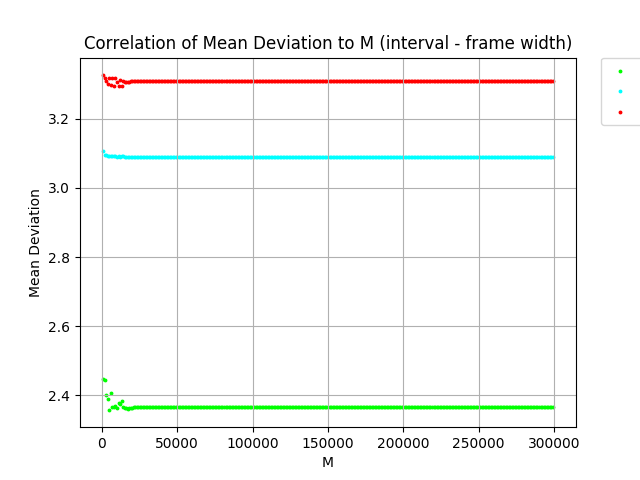
\includegraphics[width=0.55\linewidth]{./data/PriceAndTweets/ErrorVsTweetsN_1000to300000.png}
   	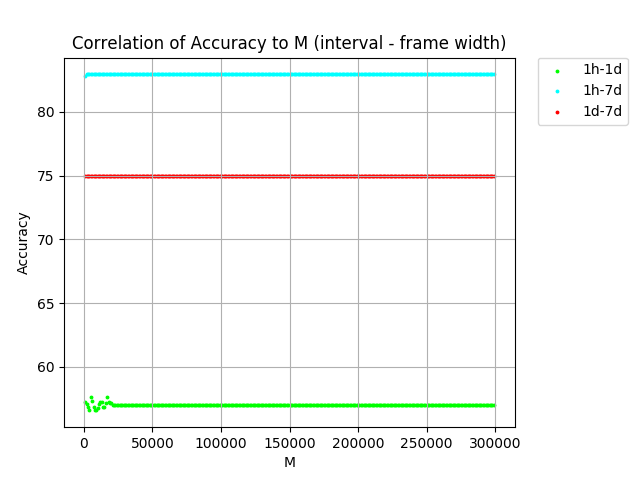
\includegraphics[width=0.55\linewidth]{./data/PriceAndTweets/AccuracyVsTweetsN_1000to300000.png}
   	\captionof{figure}{Performance of predictions (done by using combined data) for large values of M (partition amount in the tweet vector).}
   	\label{pricesandtweetsupto300000}
   \end{minipage}%
   \hfill
   
   
   \subsubsection{Using Twitter data}
   In the Figure \ref{tweetsupto300000} you can see the performance of predictions for larger number of partitions in the tweets vector. The predictions shown in these figures are predictions made using only Twitter data, or, in other words, only tweets vector was used as input for predictions.
   
   
   
   \begin{minipage}{\linewidth}
   	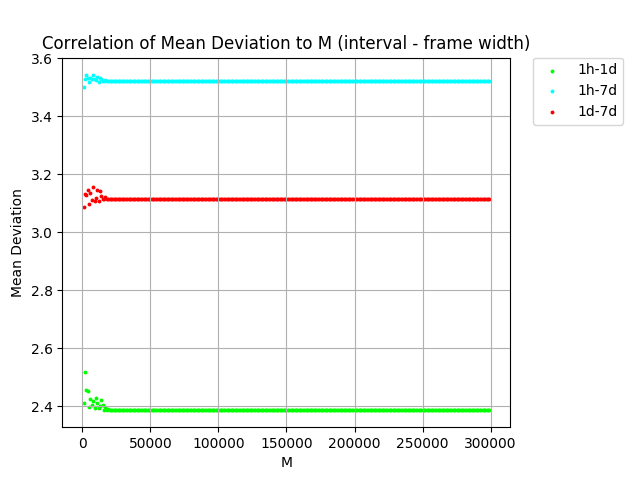
\includegraphics[width=0.57\linewidth]{./data/Tweets/ErrorVsTweetsN_1000to300000.png}
   	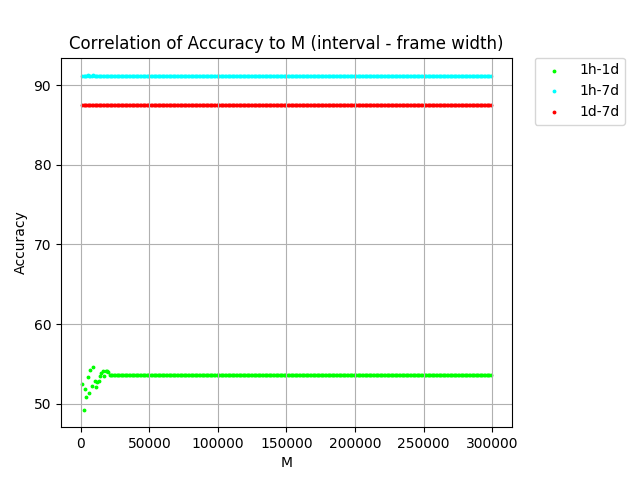
\includegraphics[width=0.53\linewidth]{./data/Tweets/AccuracyVsTweetsN_1000to300000.png}
   	\captionof{figure}{Performance of predictions (done by using only Twitter data) for large values of M (partition amount in the tweet vector).}
   	\label{tweetsupto300000}
   \end{minipage}%
   \hfill
\end{document}
